\documentclass{../../zirkelblatt}

\usepackage{geometry}
\geometry{tmargin=0.5cm,bmargin=0.5cm,lmargin=1cm,rmargin=1cm}

\pagestyle{empty}

\begin{document}

\newcommand{\vorderseite}{
  \begin{minipage}[t][4cm][t]{7.6cm}
    \begin{center}
      \textsf{Die Eulersche Zahl~$e$, eine transzendente Zahl}
      \vspace{0.6em}
      \tiny

      718 281 8284 590 452 3536 028 747 1352 662 497 7572 470 936 9995 

      957 496 6967 627 724 0766 303 535 4759 457 138 2178 525 166 4274 

      274 663 9193 200 305 9921 817 413 5966 290 435 7290 033 429 5260 

      595 630 7381 323 286 2794 349 076 3233 829 880 7531 952 510 1901 

      157 383 4187 930 702 1540 891 499 3488 416 750 9244 761 460 6680 

      822 648 0016 847 741 1853 742 345 4424 371 075 3907 774 499 2069 

      551 702 7618 386 062 6133 138 458 3000 752 044 9338 265 602 9760 

      673 711 3200 709 328 7091 274 437 4704 723 069 6977 209 310 1416 
    \end{center}

    \centering%
    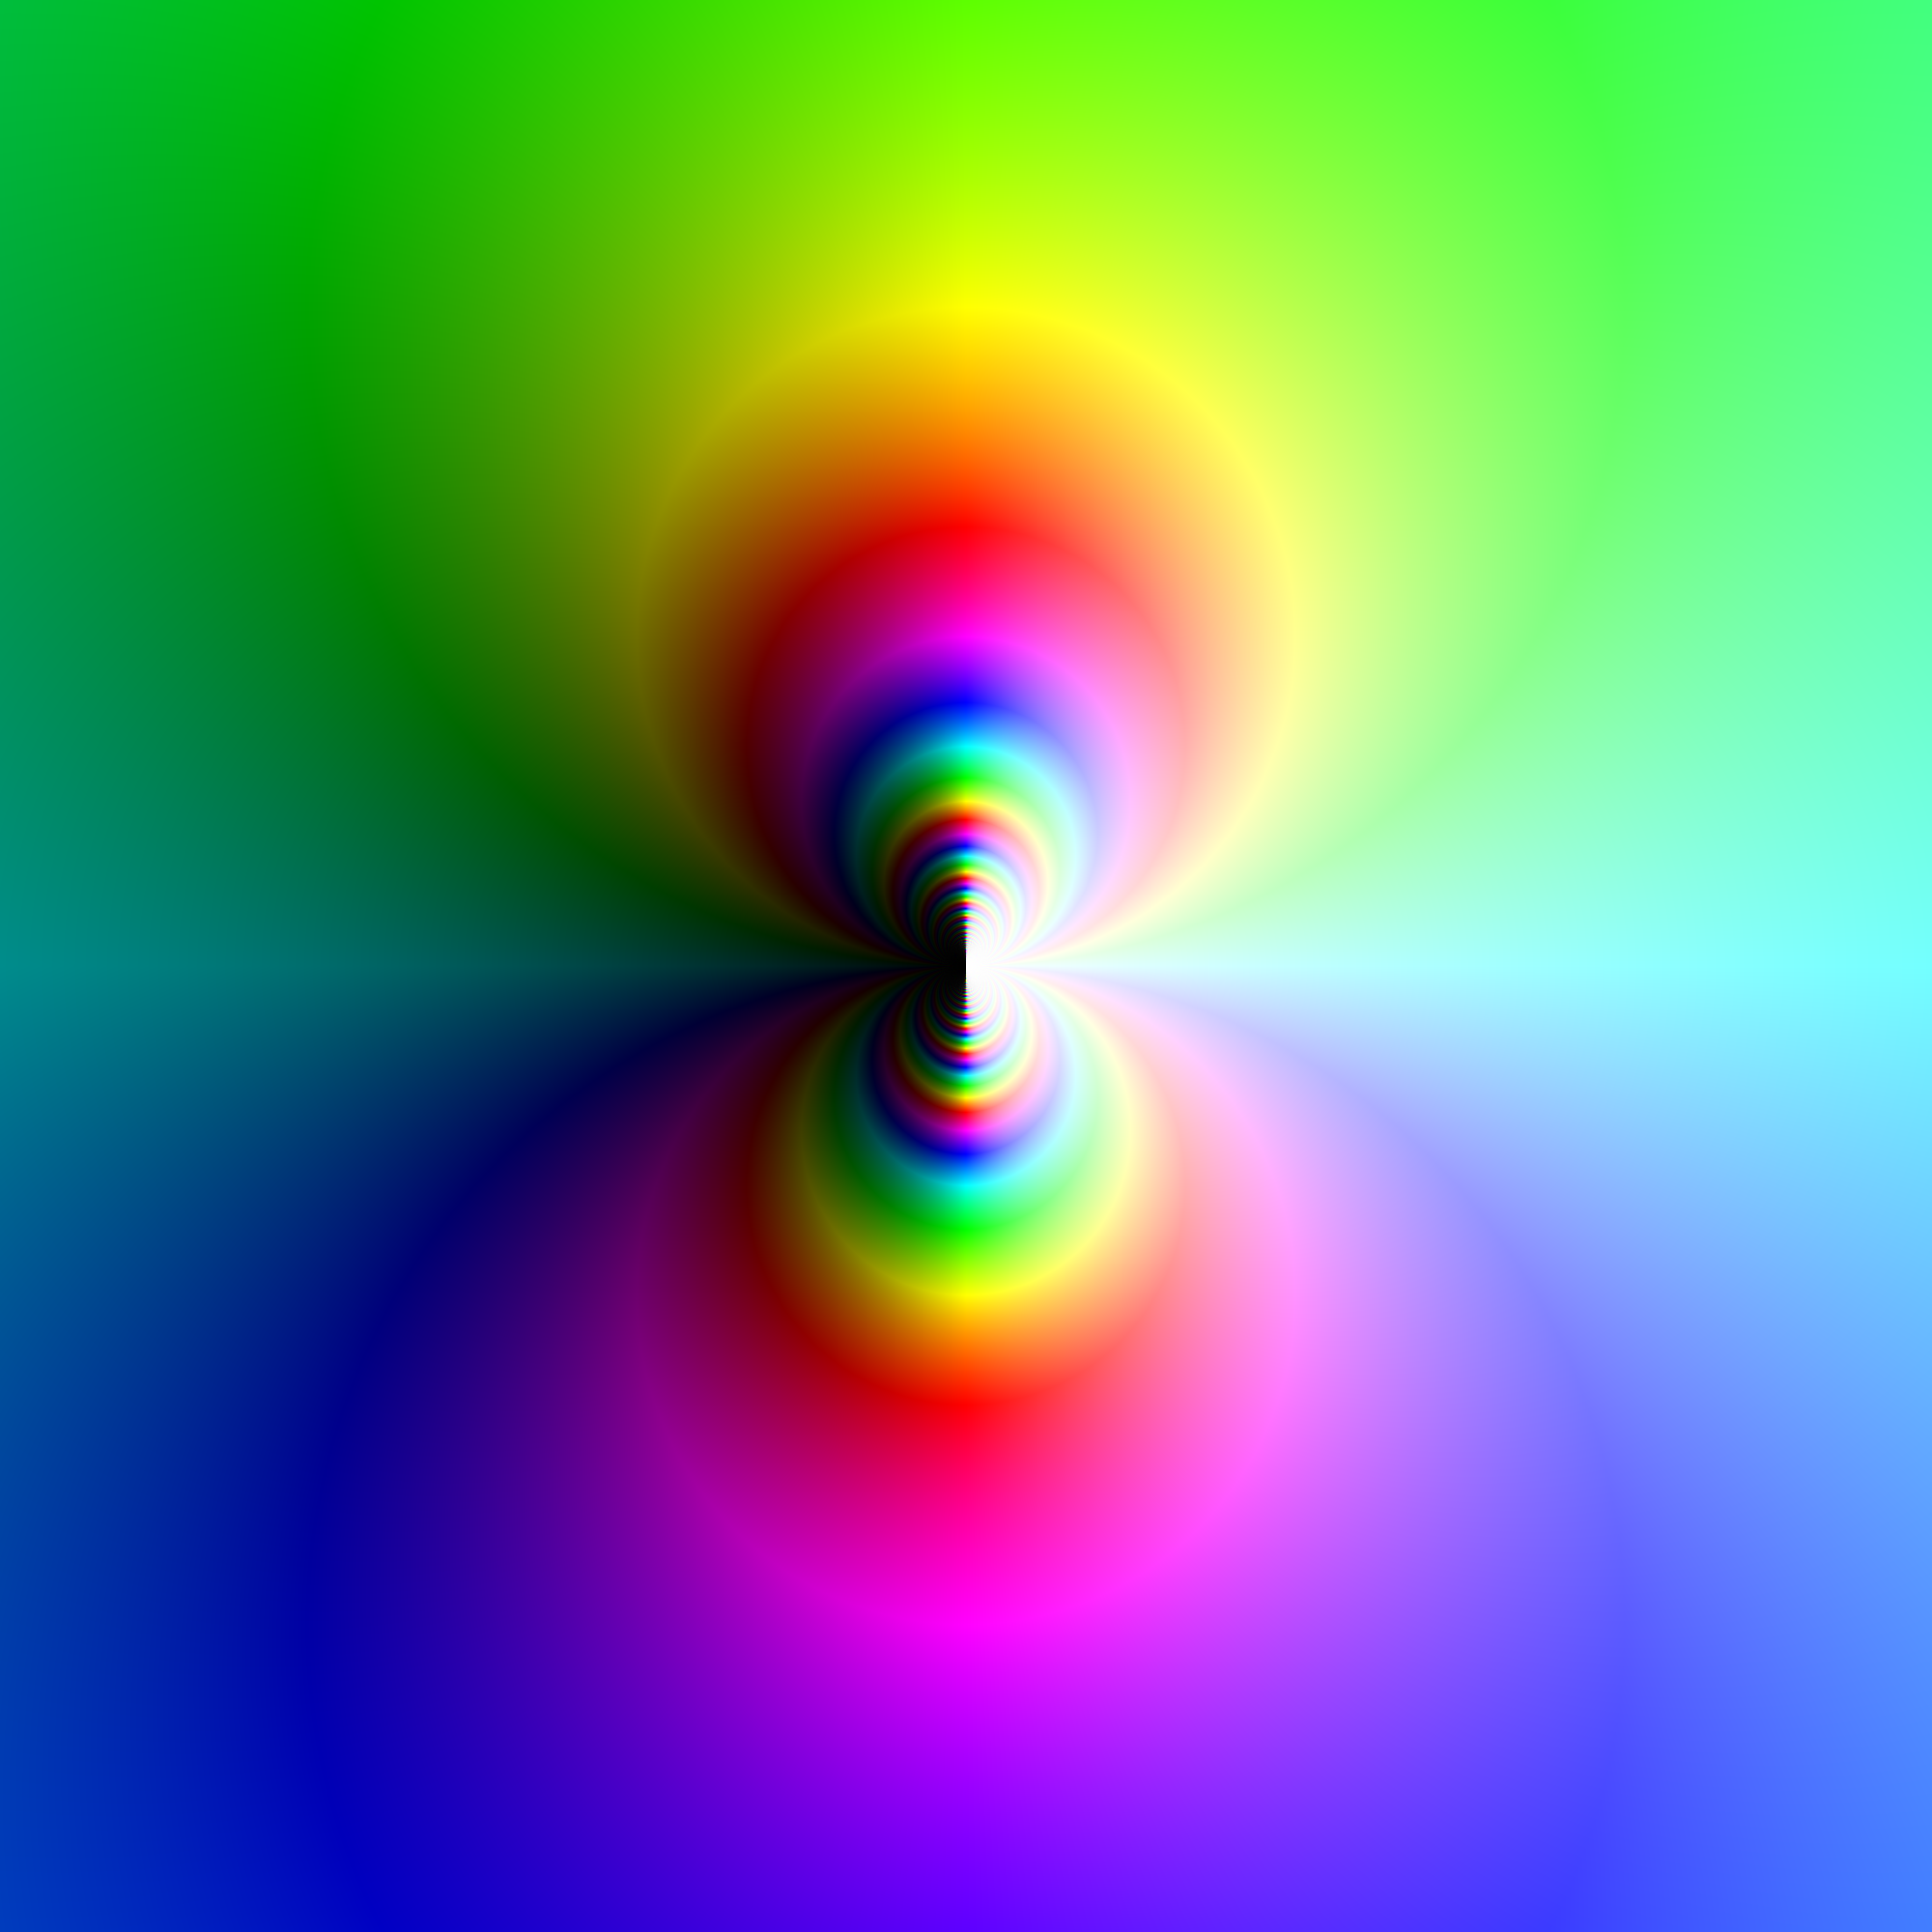
\includegraphics[width=0.95\textwidth,height=1cm]{essential-singularity}
    \par
  \end{minipage}
}

\newcommand{\rueckseite}{
  \begin{minipage}[t][4cm][t]{7.6cm}
    \phantom{A}
    \vspace{-0.3em}
    \tiny

    Die Eulersche Zahl~$e$ ist ungefähr 3: $e = 2{,}718\ldots$
    Sie findet bei der Beschreibung \textbf{exponentieller Prozesse} Anwendung.
    Wenn~$n$ Mathematikerinnen und Mathematiker ihre Namen auf Zettel schreiben, die Zettel mischen und dann
    zufällig je einen Zettel ziehen, ist im Grenzwert~$n \to \infty$ die
    Wahrscheinlichkeit, dass niemand seinen eigenen Zettel zieht, genau~$1/e$.
    Die Zahl~$e$ ist \textbf{irrational}, lässt sich also nicht als Bruch
    zweier ganzer Zahlen schreiben. Außerdem ist~$e$ sogar
    \textbf{trans\-zen\-dent}, also keine Lösung einer Polynomgleichung.
    Erstaunlicherweise ist die Kettenbruchentwicklung von~$e$ aber völlig
    regelmäßig. Die rechts angegebene Näherung ist auf
    18\,457\,734\,525\,360\,901\,453\,873\,570 Dezimalen korrekt.
    \scalebox{0.7}{\begin{minipage}{0.71\textwidth}
      \[ e = 1 + 1 + \frac{1}{1 + \frac{1}{2 + \frac{1}{1 + \frac{1}{1 +
      \frac{1}{4 + \frac{1}{1 + \frac{1}{1 + \frac{1}{6 + \cdots}}}}}}}} \]
    \end{minipage}\begin{minipage}{0.71\textwidth}
    \begin{align*}
      e &= \frac{1}{1} + \frac{1}{1} + \frac{1}{1\cdot2} + \frac{1}{1\cdot2\cdot3} + \cdots \\
      e &= \lim_{n\to\infty} (1+\tfrac{1}{n})^n \approx
      (1+9^{-4^{7\cdot6}})^{3^{2^{85}}} \\
      0 &= e^{i \pi} + 1
    \end{align*}\end{minipage}}
  \end{minipage}
}

\vorderseite\hfill\vorderseite
\vfill
\vorderseite\hfill\vorderseite
\vfill
\vorderseite\hfill\vorderseite
\vfill
\vorderseite\hfill\vorderseite
\vfill
\vorderseite\hfill\vorderseite

\newpage

\fontfamily{kurier}\selectfont

\rueckseite\hfill\rueckseite
\vfill
\rueckseite\hfill\rueckseite
\vfill
\rueckseite\hfill\rueckseite
\vfill
\rueckseite\hfill\rueckseite
\vfill
\rueckseite\hfill\rueckseite

\end{document}
